% Created 2012-04-01 Dom 20:56
\documentclass[11pt]{article}
\usepackage[utf8]{inputenc}
\usepackage[T1]{fontenc}
\usepackage{graphicx}
\usepackage{longtable}
\usepackage{hyperref}


\title{experiments}
\author{Rafael Lemes Beirigo}
\date{01 abril 2012}

\begin{document}

\maketitle

\setcounter{tocdepth}{3}
\tableofcontents
\vspace*{1cm}
\centerline{\includegraphics[width=10em]{/home/rafaelbeirigo/ql/experiments/02/w.png}}


\section{00}
\label{sec-1}


\subsection{O quê: Reprodução do artigo}
\label{sec-1.1}

\subsection{Resultado: diverso do esperado}
\label{sec-1.2}

   O Q-Learning apresentou um desempenho extremamente melhor do que o PRQL.
   Houve um problema: não estava zerando as Q-Tables (QLearning e PRQLearning)
         

\section{01}
\label{sec-2}

\centerline{\includegraphics[width=10em]{/home/rafaelbeirigo/ql/experiments/02/w.png}}

Repetição de 00 após correção do problema
Resultado: PRQL tem o mesmo comportamento de QL, só um pouco pior.
Hipótese: não está utilizando as políticas antigas


\section{02 QL vs PRQL no mundo 05x05}
\label{sec-3}

\centerline{\includegraphics[width=10em]{/home/rafaelbeirigo/ql/experiments/02/w.png}}

Motivo: queria rodar o PRQL sem a parte PR, ou seja, só utilizando
QLearning, pra ver se estava tudo OK
Nesse experimento, NÃO utilizava pi-reuse, somente QL


\section{03 Mesmo experimento de 02, só que para o mundo 06x06}
\label{sec-4}



\section{04 Mesmo experimento de 02, só que para a task omega do artigo}
\label{sec-5}

\centerline{\includegraphics[width=10em]{/home/rafaelbeirigo/ql/experiments/04/w.png}}

\subsection{Resultado:}
\label{sec-5.1}

   PRQL e QL apresentaram desempenhos compatíveis, o que era esperado


\section{05 Repetindo 04, só que dessa vez ativando o pi-reuse}
\label{sec-6}

\centerline{\includegraphics[width=10em]{/home/rafaelbeirigo/ql/experiments/05/w.png}}

  Sucesso: PRQL acelerou QLearning


\section{06 Repetindo 05 para task omega do artigo reutilizando políticas 2, 3 e 5 (são as que mais ajudam o agente)}
\label{sec-7}

\centerline{\includegraphics[width=10em]{/home/rafaelbeirigo/ql/experiments/06/w.png}}

  Problema: plotando W[ 1]


\section{07 Repetindo 06}
\label{sec-8}

\centerline{\includegraphics[width=10em]{/home/rafaelbeirigo/ql/experiments/07/w.png}}

  Problema: plotando W[ 1]


\section{08 Repetindo 06, mas reutilizando somente a política ótima}
\label{sec-9}

\centerline{\includegraphics[width=10em]{/home/rafaelbeirigo/ql/experiments/08/w.png}}

  Problema: plotando W[ 1]


\section{09 Repetindo 02, após correção do acúmulo de recompensas médias por episódio}
\label{sec-10}

\centerline{\includegraphics[width=10em]{/home/rafaelbeirigo/ql/experiments/09/w.png}}

Problema: reutilizando políticas subótimas


\section{10 Repetindo 09, mas reutilizando uma política ótima para o problema de chegar}
\label{sec-11}

  à localização oposta (pior política que poderia reutilizar)
\centerline{\includegraphics[width=10em]{/home/rafaelbeirigo/ql/experiments/10/w.png}}

Problema: reutilizando políticas subótimas


\section{11 Resolver task omega utilizando pols. 2,3,4,5}
\label{sec-12}

\centerline{\includegraphics[width=10em]{/home/rafaelbeirigo/ql/experiments/11/w.png}}

Problema: reutilizando políticas subótimas


\section{12 Repetindo 11 reutilizando somente a policy obtida em 11 pelo}
\label{sec-13}

  QLearning (ótima para o problema)
\centerline{\includegraphics[width=10em]{/home/rafaelbeirigo/ql/experiments/12/w.png}}

Problema: reutilizando políticas subótimas


\section{13 Repetindo 12, só que chamei o solveMDP\ldots{} pra criar os arquivos (tirar a dúvida se}
\label{sec-14}

  arquivos estão corretos)
\centerline{\includegraphics[width=10em]{/home/rafaelbeirigo/ql/experiments/13/w.png}}

Problema: reutilizando políticas subótimas


\section{14 Repetição do 13, só que agora utilizando a política ótima}
\label{sec-15}

\centerline{\includegraphics[width=10em]{/home/rafaelbeirigo/ql/experiments/14/w.png}}



\section{15 Obtenção de política para task 1}
\label{sec-16}

\centerline{\includegraphics[width=10em]{/home/rafaelbeirigo/ql/experiments/15/w.png}}

  Consumo de tempo: \~{} 10'


\section{16 Obtenção de política para task 2}
\label{sec-17}

\centerline{\includegraphics[width=10em]{/home/rafaelbeirigo/ql/experiments/16/w.png}}

  Consumo de tempo: \~{} 10'


\section{17 Obtenção de política para task 3}
\label{sec-18}

\centerline{\includegraphics[width=10em]{/home/rafaelbeirigo/ql/experiments/17/w.png}}

  Consumo de tempo: \~{} 10'


\section{18 Obtenção de política para task 4}
\label{sec-19}

\centerline{\includegraphics[width=10em]{/home/rafaelbeirigo/ql/experiments/18/w.png}}

  Consumo de tempo: \~{} 10'


\section{19 Obtenção de política para task 5}
\label{sec-20}

\centerline{\includegraphics[width=10em]{/home/rafaelbeirigo/ql/experiments/19/w.png}}

  Consumo de tempo: \~{} 10'


\section{20 Resolver task omega utilizando pols. 2,3,4,5 (Repetição do 11)}
\label{sec-21}

\centerline{\includegraphics[width=10em]{/home/rafaelbeirigo/ql/experiments/20/w.png}}



\section{21 Resolver task omega utilizando pols. 2,3,4}
\label{sec-22}

\centerline{\includegraphics[width=10em]{/home/rafaelbeirigo/ql/experiments/21/w.png}}



\section{22 Resolver task omega utilizando pols. 1,2,3,4}
\label{sec-23}

\centerline{\includegraphics[width=10em]{/home/rafaelbeirigo/ql/experiments/22/w.png}}



\section{23 Repetição do 02}
\label{sec-24}



\section{24 Repetição do 22}
\label{sec-25}



\section{25 Repetição do 20}
\label{sec-26}



\section{26 Repetição do 21}
\label{sec-27}


\end{document}
